\documentclass[twoside,11pt]{article}

% ? Specify used packages
\usepackage{graphicx}        %  Use this one for final production.
% \usepackage[draft]{graphicx} %  Use this one for drafting.
% ? End of specify used packages

\pagestyle{myheadings}

% -----------------------------------------------------------------------------
% ? Document identification
% Fixed part
\newcommand{\stardoccategory}  {STARLINK User Note}
\newcommand{\stardocinitials}  {SUN}
\newcommand{\stardocsource}    {sun\stardocnumber}

% Variable part - replace [xxx] as appropriate.
\newcommand{\stardocnumber}    {237.4}
\newcommand{\stardocauthors}   {A.~Allan \& Malcolm J. Currie}
\newcommand{\stardocdate}      {2010 September 7}
\newcommand{\stardoctitle}     {DATACUBE --- An IFS datacube manipulation package}
\newcommand{\stardocversion}   {Version 1.3}
\newcommand{\stardocmanual}    {User's Manual}
\newcommand{\stardocabstract}  {
\htmlref{DATACUBE}{DATACUBE} is a package which includes the IFU Data Product Cookbook (\xref{SC/16}{sc16}{}), and a collection of example shell scripts for IFS data cube manipulation.
}

% ? End of document identification
% -----------------------------------------------------------------------------

% +
%  Name:
%     sc.tex
%
%  Purpose:
%     Template for Starlink Cookbook (SC) documents.
%     Refer to SUN/199
%
%  Authors:
%     AJC: A.J.Chipperfield (Starlink, RAL)
%     BLY: M.J.Bly (Starlink, RAL)
%
%  History:
%     16-JUN-1997 (BLY):
%        Original, based on SUN/SG templates.
%     {Add further history here}
%
% -

\newcommand{\stardocname}{\stardocinitials /\stardocnumber}
\markboth{\stardocname}{\stardocname}
\setlength{\textwidth}{160mm}
\setlength{\textheight}{230mm}
\setlength{\topmargin}{-2mm}
\setlength{\oddsidemargin}{0mm}
\setlength{\evensidemargin}{0mm}
\setlength{\parindent}{0mm}
\setlength{\parskip}{\medskipamount}
\setlength{\unitlength}{1mm}

% -----------------------------------------------------------------------------
%  Hypertext definitions.
%  ======================
%  These are used by the LaTeX2HTML translator in conjunction with star2html.

%  Comment.sty: version 2.0, 19 June 1992
%  Selectively in/exclude pieces of text.
%
%  Author
%    Victor Eijkhout                                      <eijkhout@cs.utk.edu>
%    Department of Computer Science
%    University Tennessee at Knoxville
%    104 Ayres Hall
%    Knoxville, TN 37996
%    USA

%  Do not remove the %begin{latexonly} and %end{latexonly} lines (used by
%  star2html to signify raw TeX that latex2html cannot process).
%begin{latexonly}
\makeatletter
\def\makeinnocent#1{\catcode`#1=12 }
\def\csarg#1#2{\expandafter#1\csname#2\endcsname}

\def\ThrowAwayComment#1{\begingroup
    \def\CurrentComment{#1}%
    \let\do\makeinnocent \dospecials
    \makeinnocent\^^L% and whatever other special cases
    \endlinechar`\^^M \catcode`\^^M=12 \xComment}
{\catcode`\^^M=12 \endlinechar=-1 %
 \gdef\xComment#1^^M{\def\test{#1}
      \csarg\ifx{PlainEnd\CurrentComment Test}\test
          \let\html@next\endgroup
      \else \csarg\ifx{LaLaEnd\CurrentComment Test}\test
            \edef\html@next{\endgroup\noexpand\end{\CurrentComment}}
      \else \let\html@next\xComment
      \fi \fi \html@next}
}
\makeatother

\def\includecomment
 #1{\expandafter\def\csname#1\endcsname{}%
    \expandafter\def\csname end#1\endcsname{}}
\def\excludecomment
 #1{\expandafter\def\csname#1\endcsname{\ThrowAwayComment{#1}}%
    {\escapechar=-1\relax
     \csarg\xdef{PlainEnd#1Test}{\string\\end#1}%
     \csarg\xdef{LaLaEnd#1Test}{\string\\end\string\{#1\string\}}%
    }}

%  Define environments that ignore their contents.
\excludecomment{comment}
\excludecomment{rawhtml}
\excludecomment{htmlonly}

%  Hypertext commands etc. This is a condensed version of the html.sty
%  file supplied with LaTeX2HTML by: Nikos Drakos <nikos@cbl.leeds.ac.uk> &
%  Jelle van Zeijl <jvzeijl@isou17.estec.esa.nl>. The LaTeX2HTML documentation
%  should be consulted about all commands (and the environments defined above)
%  except \xref and \xlabel which are Starlink specific.

\newcommand{\htmladdnormallinkfoot}[2]{#1\footnote{#2}}
\newcommand{\htmladdnormallink}[2]{#1}
\newcommand{\htmladdimg}[1]{}
\newcommand{\hyperref}[4]{#2\ref{#4}#3}
\newcommand{\htmlref}[2]{#1}
\newcommand{\htmlimage}[1]{}
\newcommand{\htmladdtonavigation}[1]{}

% Define commands for HTML-only or LaTeX-only text.
\newenvironment{latexonly}{}{}
\newcommand{\html}[1]{}
\newcommand{\latex}[1]{#1}

% Use latex2html 98.2.
\newcommand{\latexhtml}[2]{#1}

%  Provide CSS support.
\newcommand{\htmlsetstyle}[3][]{}
\newcommand{\htmladdtostyle}[3][]{}

%  Starlink cross-references and labels.
\newcommand{\xref}[3]{#1}
\newcommand{\xlabel}[1]{}

%  LaTeX2HTML symbol.
\newcommand{\latextohtml}{{\bf LaTeX}{2}{\tt{HTML}}}

%  Define command to re-centre underscore for Latex and leave as normal
%  for HTML (severe problems with \_ in tabbing environments and \_\_
%  generally otherwise).
\renewcommand{\_}{\texttt{\symbol{95}}}
%\newcommand{\setunderscore}{\renewcommand{\_}{{\tt\symbol{95}}}}
%\latex{\setunderscore}

%  Redefine the \tableofcontents command. This procrastination is necessary
%  to stop the automatic creation of a second table of contents page
%  by latex2html.
\newcommand{\latexonlytoc}[0]{\tableofcontents}

% Figure environment. Defined for latex2html. #1 is postscript file
% #2 the qualifiers, #3 the gif file, #4 the label, #5 the caption.
\newcommand{\myfig} [5] {
  \begin{figure}
    \centering\includegraphics[#2]{#1}
    \typeout{#1 inserted on page \arabic{page}}
    \caption{\label{#4}#5}
  \end{figure}
  }
\begin{htmlonly}
  \newcommand{\myfig}[5]{
    \label{#4} \htmladdimg{#3}\\
    Figure: #5\\
    }
\end{htmlonly}

% -----------------------------------------------------------------------------
%  Debugging.
%  =========
%  Remove % on the following to debug links in the HTML version using Latex.

% \newcommand{\hotlink}[2]{\fbox{\begin{tabular}[t]{@{}c@{}}#1\\\hline{\footnotesize #2}\end{tabular}}}
% \renewcommand{\htmladdnormallinkfoot}[2]{\hotlink{#1}{#2}}
% \renewcommand{\htmladdnormallink}[2]{\hotlink{#1}{#2}}
% \renewcommand{\hyperref}[4]{\hotlink{#1}{\S\ref{#4}}}
% \renewcommand{\htmlref}[2]{\hotlink{#1}{\S\ref{#2}}}
% \renewcommand{\xref}[3]{\hotlink{#1}{#2 -- #3}}
%end{latexonly}
% -----------------------------------------------------------------------------
% ? Document specific \newcommand or \newenvironment commands.

% an environment for references (for the SST sstdiytopic command).
\newenvironment{refs}{\vspace{-4ex} % normally 3ex
                      \begin{list}{}{\setlength{\topsep}{0mm}
                                     \setlength{\partopsep}{0mm}
                                     \setlength{\itemsep}{0mm}
                                     \setlength{\parsep}{0mm}
                                     \setlength{\leftmargin}{1.5em}
                                     \setlength{\itemindent}{-\leftmargin}
                                     \setlength{\labelsep}{0mm}
                                     \setlength{\labelwidth}{0mm}}
                                 }{\end{list}}


% Shorthands for hypertext links.
% -------------------------------

\newcommand{\DATACUBE}{{\footnotesize DATACUBE}\normalsize}
\newcommand{\FIGARO}{{\footnotesize FIGARO}\normalsize}
\newcommand{\FIGAROref}{\xref{\FIGARO}{sun86}{}}
\newcommand{\KAPPA}{{\footnotesize KAPPA}\normalsize}
\newcommand{\KAPPAref}{\xref{\KAPPA}{sun95}{}}

% +
%  Name:
%     SST.TEX

%  Purpose:
%     Define LaTeX commands for laying out Starlink routine descriptions.

%  Language:
%     LaTeX

%  Type of Module:
%     LaTeX data file.

%  Description:
%     This file defines LaTeX commands which allow routine documentation
%     produced by the SST application PROLAT to be processed by LaTeX and
%     by LaTeX2html. The contents of this file should be included in the
%     source prior to any statements that make of the sst commnds.

%  Notes:
%     The commands defined in the style file html.sty provided with LaTeX2html
%     are used. These should either be made available by using the appropriate
%     sun.tex (with hypertext extensions) or by putting the file html.sty
%     on your TEXINPUTS path (and including the name as part of the
%     documentstyle declaration).

%  Authors:
%     RFWS: R.F. Warren-Smith (STARLINK)
%     PDRAPER: P.W. Draper (Starlink - Durham University)

%  History:
%     10-SEP-1990 (RFWS):
%        Original version.
%     10-SEP-1990 (RFWS):
%        Added the implementation status section.
%     12-SEP-1990 (RFWS):
%        Added support for the usage section and adjusted various spacings.
%     8-DEC-1994 (PDRAPER):
%        Added support for simplified formatting using LaTeX2html.
%     {enter_further_changes_here}

%  Bugs:
%     {note_any_bugs_here}

% -

%  Define length variables.
\newlength{\sstbannerlength}
\newlength{\sstcaptionlength}
\newlength{\sstexampleslength}
\newlength{\sstexampleswidth}

%  Define a \tt font of the required size.
\newfont{\ssttt}{cmtt10 scaled 1095}

%  Define a command to produce a routine header, including its name,
%  a purpose description and the rest of the routine's documentation.
\newcommand{\sstroutine}[3]{
   \goodbreak
   \rule{\textwidth}{0.5mm}
   \vspace{-7ex}
   \newline
   \settowidth{\sstbannerlength}{{\Large {\bf #1}}}
   \setlength{\sstcaptionlength}{\textwidth}
   \setlength{\sstexampleslength}{\textwidth}
   \addtolength{\sstbannerlength}{0.5em}
   \addtolength{\sstcaptionlength}{-2.0\sstbannerlength}
   \addtolength{\sstcaptionlength}{-5.0pt}
   \settowidth{\sstexampleswidth}{{\bf Examples:}}
   \addtolength{\sstexampleslength}{-\sstexampleswidth}
   \parbox[t]{\sstbannerlength}{\flushleft{\Large {\bf #1}}}
   \parbox[t]{\sstcaptionlength}{\center{\Large #2}}
   \parbox[t]{\sstbannerlength}{\flushright{\Large {\bf #1}}}
   \begin{description}
      #3
   \end{description}
}

%  Format the description section.
\newcommand{\sstdescription}[1]{\item[Description:] #1}

%  Format the usage section.
\newcommand{\sstusage}[1]{\item[Usage:] \mbox{} \\[1.3ex] {\ssttt #1}}


%  Format the invocation section.
\newcommand{\sstinvocation}[1]{\item[Invocation:]\hspace{0.4em}{\tt #1}}

%  Format the arguments section.
\newcommand{\sstarguments}[1]{
   \item[Arguments:] \mbox{} \\
   \vspace{-3.5ex}
   \begin{description}
      #1
   \end{description}
}


%  Format the returned value section (for a function).
\newcommand{\sstreturnedvalue}[1]{
   \item[Returned Value:] \mbox{} \\
   \vspace{-3.5ex}
   \begin{description}
      #1
   \end{description}
}

%  Format the parameters section (for an application).
\newcommand{\sstparameters}[1]{
   \item[Parameters:] \mbox{} \\
   \vspace{-3.5ex}
   \begin{description}
      #1
   \end{description}
}

%  Format the examples section.
\newcommand{\sstexamples}[1]{
   \item[Examples:] \mbox{} \\
   \vspace{-3.5ex}
   \begin{description}
      #1
   \end{description}
}

%  Define the format of a subsection in a normal section.
\newcommand{\sstsubsection}[1]{ \item[{#1}] \mbox{} \\}

%  Define the format of a subsection in the examples section.
\newcommand{\sstexamplesubsection}[2]{\sloppy
\item[\parbox{\sstexampleslength}{\ssttt #1}] \mbox{} \\ #2 }

%  Format the notes section.
\newcommand{\sstnotes}[1]{\item[Notes:] \mbox{} \\[1.3ex] #1}

%  Provide a general-purpose format for additional (DIY) sections.
\newcommand{\sstdiytopic}[2]{\item[{\hspace{-0.35em}#1\hspace{-0.35em}:}] \mbox{} \\[1.3ex] #2}

%  Format the implementation status section.
\newcommand{\sstimplementationstatus}[1]{
   \item[{Implementation Status:}] \mbox{} \\[1.3ex] #1}

%  Format the bugs section.
\newcommand{\sstbugs}[1]{\item[Bugs:] #1}

%  Format a list of items while in paragraph mode, and where there
%  is a heading, thus the negative vertical space is not needed.
\newcommand{\ssthitemlist}[1]{
  \mbox{} \\
  \vspace{-8.0ex}
  \begin{itemize}
     #1
  \end{itemize}
}
%  Format a list of items while in paragraph mode.
\newcommand{\sstitemlist}[1]{
  \mbox{} \\
  \vspace{-3.5ex}
  \begin{itemize}
     #1
  \end{itemize}
}

%  Define the format of an item.
\newcommand{\sstitem}{\item}

%  Now define html equivalents of those already set. These are used by
%  latex2html and are defined in the html.sty files.
\begin{htmlonly}

%  Re-define \ssttt.
   \newcommand{\ssttt}{\tt}

%  sstroutine.
   \newcommand{\sstroutine}[3]{
      \subsection{#1\xlabel{#1}-\label{#1}#2}
      \begin{description}
         #3
      \end{description}
   }

%  sstdescription
   \newcommand{\sstdescription}[1]{\item[Description:]
      \begin{description}
         #1
      \end{description}
   }

%  sstusage
   \newcommand{\sstusage}[1]{\item[Usage:]
      \begin{description}
         {\ssttt #1}
      \end{description}
      \\
   }

%  sstinvocation
   \newcommand{\sstinvocation}[1]{\item[Invocation:]
      \begin{description}
         {\ssttt #1}
      \end{description}
   }

%  sstarguments
   \newcommand{\sstarguments}[1]{
      \item[Arguments:]
      \begin{description}
         #1
      \end{description}
   }

%  sstreturnedvalue
   \newcommand{\sstreturnedvalue}[1]{
      \item[Returned Value:]
      \begin{description}
         #1
      \end{description}
   }

%  sstparameters
   \newcommand{\sstparameters}[1]{
      \item[Parameters:]
      \begin{description}
         #1
      \end{description}
   }

%  sstexamples
   \newcommand{\sstexamples}[1]{
      \item[Examples:]
      \begin{description}
         #1
      \end{description}
   }

%  sstsubsection
   \newcommand{\sstsubsection}[1]{\item[{#1}]}

%  sstexamplesubsection
   \newcommand{\sstexamplesubsection}[2]{\item[{\ssttt #1}] \\ #2}

%  sstnotes
   \newcommand{\sstnotes}[1]{\item[Notes:]
      \begin{description}
         #1
      \end{description}
   }

%  sstdiytopic
   \newcommand{\sstdiytopic}[2]{\item[{#1}]
      \begin{description}
         #2
      \end{description}
   }

%  sstimplementationstatus
   \newcommand{\sstimplementationstatus}[1]{\item[Implementation Status:]
      \begin{description}
         #1
      \end{description}
   }


%  sstitemlist
   \newcommand{\ssthitemlist}[1]{
      \begin{itemize}
         #1
      \end{itemize}
      \\
   }

   \newcommand{\sstitemlist}[1]{
      \begin{itemize}
         #1
      \end{itemize}
   }
\end{htmlonly}

%  End of "sst.tex" layout definitions.
% .
% @(#)sst.tex   1.4   95/06/06 11:46:41   96/07/05 10:28:17

% ? End of document specific commands
% -----------------------------------------------------------------------------
%  Title Page.
%  ===========
\renewcommand{\thepage}{\roman{page}}
\begin{document}
\thispagestyle{empty}

%  Latex document header.
%  ======================
\begin{latexonly}
   CCLRC / {\sc Rutherford Appleton Laboratory} \hfill {\bf \stardocname}\\
   {\large Particle Physics \& Astronomy Research Council}\\
   {\large Starlink Project\\}
   {\large \stardoccategory\ \stardocnumber}
   \begin{flushright}
   \stardocauthors\\
   \stardocdate
   \end{flushright}
   \vspace{-4mm}
   \rule{\textwidth}{0.5mm}
   \vspace{5mm}
   \begin{center}
   {\Huge\bf  \stardoctitle \\ [2.5ex]}
   \end{center}
   \vspace{5mm}

% ? Add picture here if required for the LaTeX version.
%   e.g. \includegraphics[scale=0.3]{filename}
   \begin{center}
   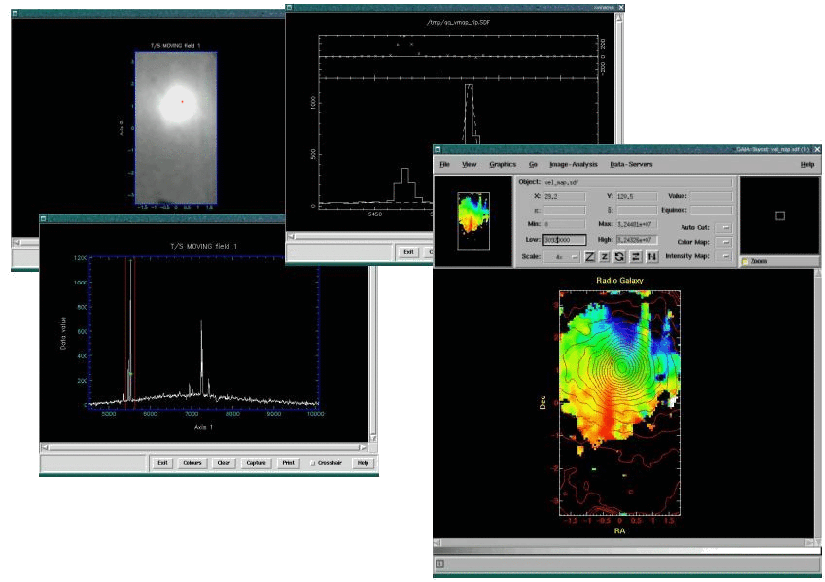
\includegraphics[scale=0.6]{sun237_cover}
   \end{center}
% ? End of picture

% ? Heading for abstract if used.
   \vspace{5mm}
   \begin{center}
      {\Large\bf Abstract}
   \end{center}
% ? End of heading for abstract.
\end{latexonly}

%  HTML documentation header.
%  ==========================
\begin{htmlonly}
   \xlabel{}
   \begin{rawhtml} <H1> \end{rawhtml}
      \stardoctitle\\
      \stardocversion\\
      \stardocmanual
   \begin{rawhtml} </H1> \end{rawhtml}

% ? Add picture here if required for the hypertext version.
%   e.g. \includegraphics[scale=0.7]{filename.ps}
   \htmladdimg{sun237_cover.png}

% ? End of picture

   \begin{rawhtml} <P> <I> \end{rawhtml}
   \stardoccategory\ \stardocnumber \\
   \stardocauthors \\
   \stardocdate
   \begin{rawhtml} </I> </P> <H3> \end{rawhtml}
      \htmladdnormallink{CCLRC}{http://www.cclrc.ac.uk} /
      \htmladdnormallink{Rutherford Appleton Laboratory}
                        {http://www.cclrc.ac.uk/ral} \\
      \htmladdnormallink{Particle Physics \& Astronomy Research Council}
                        {http://www.pparc.ac.uk} \\
   \begin{rawhtml} </H3> <H2> \end{rawhtml}
      \htmladdnormallink{Starlink Project}{http://www.starlink.ac.uk/}
   \begin{rawhtml} </H2> \end{rawhtml}
   \htmladdnormallink{\htmladdimg{source.gif} Retrieve hardcopy}
      {http://www.starlink.ac.uk/cgi-bin/hcserver?\stardocsource}\\

%  HTML document table of contents.
%  ================================
%  Add table of contents header and a navigation button to return to this
%  point in the document (this should always go before the abstract \section).
  \label{stardoccontents}
  \begin{rawhtml}
    <HR>
    <H2>Contents</H2>
  \end{rawhtml}
  \newcommand{\latexonlytoc}[0]{}
%  \htmladdtonavigation{\htmlref{\htmladdimg{sc15_cover.gif}}
%        {stardoccontents}}

% ? New section for abstract if used.
  \section{\xlabel{abstract}Abstract}
% ? End of new section for abstract
\end{htmlonly}

% -----------------------------------------------------------------------------
% ? Document Abstract. (if used)
%  ==================
\stardocabstract
% ? End of document abstract
% -----------------------------------------------------------------------------
% ? Latex document Table of Contents (if used).
%  ===========================================
 \newpage
 \vspace{3cm}

 \subsection*{Revision history}

 \begin{enumerate}
   \item 9th November 2000; Version 0.1 Original version (AA)
   \item 30th December 2000; Version 0.2 Auto-generated code prologs (AA)
   \item 2nd January 2001; Version 1.0 Release version (AA)
   \item 2005 October 20; Version 1.1 Removed applications, and improved scripts (MJC)
   \item 2006 March 10; Version 1.1 Add gridspec and velmoment, and
         used implementation status (MJC)
   \item 2008 July 2; Version 1.2 Added trendview and improved the introduction (MJC)
   \item 2010 July 13; Version 1.2 Added pvslice (MJC)

 \end{enumerate}

 \vspace{10cm}
 \copyright \underline{1999-2005} Starlink, CCLRC

 \cleardoublepage
 \begin{latexonly}
   \setlength{\parskip}{0mm}
   \latexonlytoc

   \newpage
   \listoffigures
   %\listoftables

   \setlength{\parskip}{\medskipamount}
   \markright{\stardocname}
 \end{latexonly}
% ? End of Latex document table of contents
% -----------------------------------------------------------------------------

\cleardoublepage
\newpage
\renewcommand{\thepage}{\arabic{page}}
\setcounter{page}{1}

% The main text begins here.
% -----------------------------------------------------------------------------

\section{\xlabel{sun237_intro}The Datacube Package\label{sun237_intro}}

DATACUBE\ is a collection of C-shell scripts layered on top of various
pieces of the Starlink Software Collection (SSC) for the analysis of
spectral datacubes, such as from integral-field spectrometers.  The
scripts permit graphical selection of spatial and spectral regions and
features using the cursor.

\DATACUBE\ provides facilities:
\begin{itemize}
\item to view a `white-light' image of the whole and/or part of the
      spectral range (\htmlref{{\bf squash}}{squash},
      \htmlref{{\bf passband}}{passband});
\item to view a grid of channel maps of defined spectral width
      (\htmlref{{\bf step}}{step});
\item to extract individual spectra (\htmlref{{\bf ripper}}{ripper});
\item to extract an arbitrary position-spectral slice
      (\htmlref{{\bf pvslice}}{pvslice});
\item to compare spectra (\htmlref{{\bf compare}}{compare},
      \htmlref{{\bf stacker}}{stacker});
\item to average and compare groups of spectra
      (\htmlref{{\bf multistack}}{multistack});
\item to plot a grid of spectra with spatial averaging
      (\htmlref{{\bf gridspec}}{gridspec});
\item to build a velocity map from an emission line by line
      fitting (\htmlref{{\bf velmap}}{velmap}), or by intensity-weighted
      moments (\htmlref{{\bf velmoment}}{velmoment}), or by selecting
      a cube's voxels using the values of another velocity map
      as spectral co-ordinates (\htmlref{{\bf mapbyvel}}{mapbyvel});
\item to build an emission-line strength map
      (\htmlref{{\bf peakmap}}{peakmap}); and
\item to plot multiple spectra from a cube overlaying fitted baselines
      and spectral feature mask (\htmlref{{\bf trendview}}{trendview}).
\end{itemize}

The backbone of the \DATACUBE\ Package is the \xref{IFU Data Product
Cookbook}{sc16}{} (SC/16).  This includes illustrated examples of the
\DATACUBE\ scripts, script programming tips, and lists of potentially
useful applications to manipulate and analyse cubes.

The C-Shell approach was a deliberate design decision which was made
for two main reasons: first, due to the still developing nature of
the field it is difficult to pin down exactly visualisation tasks will
be necessary, and the choice of {\tt csh} means that the existing
scripts can be easily modified by the end user to do exactly the job
required; second, after examining the Starlink Software Collection
(SSC) it was realised that a great deal of the functionality required
to analyse IFU data already existed and it would be wasteful to
re-invent the wheel by re-coding large chunks of software.

Some tasks once mature can, and should, be re-coded in FORTRAN or C,
mainly for the speed and memory advantages that this will bring. For
instance the \htmlref{{\bf velmap}}{velmap} script as implemented is
rather slow and memory intensive, it seems likely that this will be
the first candidate to be re-coded in a lower-level language.

Hopefully, while I haven't managed to think of everything, there is
enough ground work here so that the approach to solving your data
visualisation or data cube manipulation problem is obvious, even if
the package doesn't have a script or application to do exactly what
you require.

While this document contains the detailed descriptions of the shell
scripts included with the package, the ``how to'' information
detailing their use can be found in \xref{SC/16}{sc16}{}.

I would welcome comments, criticisms, contributions and corrections to
the package once people start to figure out what they want to do with
this sort of data.  Comments can be sent either to the authors at
\htmladdnormallink{{\tt aa@astro.ex.ac.uk}}{mailto:aa@astro.ex.ac.uk} or
\htmladdnormallink{{\tt mjc@star.rl.ac.uk}}{mailto:mjc@star.rl.ac.uk} or
to the Starlink software librarian
\htmladdnormallink{{\tt starlink@jiscmail.ac.uk}}{mailto:starlink@jiscmail.ac.uk}.

\section{\xlabel{sun237_starting}Setting up the applications\label{sun237_starting}}

After sourcing the Starlink {\tt /star/etc/login} and {\tt
/star/etc/cshrc} files the {\tt datacube} command will make the
datacube package scripts available to you, the following
message (or one much like it!) should appear

\small\begin{verbatim}
   % datacube

      DATACUBE applications are now available -- (Version 1.2)
       Support is available by e-mailing starlink@jiscmail.ac.uk

           Type cubehelp for help on DATACUBE commands.
      Type 'showme sun237' to browse the hypertext documentation
      or 'showme sc16' to consult the IFU data product cookbook.

   %
\end{verbatim}\normalsize

at this point you can test whether the datacube package has been
correctly installed by typing

\small\begin{verbatim}
   % datacube_test
\end{verbatim}\normalsize

which will run the test script for the package. If the script does not
run correctly you should consult your Starlink system administrator.

It should be noted that there are a great many useful applications
available in other Starlink packages that will assist you in dealing
with your IFU data (see \xref{SC/16}{sc16}{} for details), so you may,
at the very minimum, wish to setup the \xref{KAPPA}{sun95}{}
applications with the {\tt kappa} command

\small\begin{verbatim}
   % kappa

        KAPPA commands are now available -- (Version 1.12)

        Type kaphelp for help on KAPPA commands.
        Type 'showme sun95' to browse the hypertext documentation.

        NOTE, several applications have had major changes made to their
        parameter lists. See the 'Release Notes' section of SUN/95 for
        details.
   %
\end{verbatim}\normalsize

\section*{\xlabel{sun237_acks}Acknowledgments\label{sun237_acks}}

In compiling this document I (AA) have again depended heavily on the help
of many people in the IFS community. However, special thanks should go
to \htmladdnormallink{Rachel
Johnston}{http://www.ast.cam.ac.uk/~raj/}, \htmladdnormallink{Jeremy
Allington-Smith}{http://star-www.dur.ac.uk:80/~jra/},
\htmladdnormallink{James Turner}{mailto:J.E.H.Turner@durham.ac.uk} and
\htmladdnormallink{Frank Valdes}{http://www.noao.edu/noao/scistaff/valdes.html} for their
co-operation and contributions.

\newpage
\appendix
\section{Descriptions of Individual Applications}
\label{sun237_appendix_descriptions}


\sstroutine{
   compare
}{
   Compares multiple extracted spectra from a three-dimensional IFU NDF
}{
   \sstdescription{
      This shell script
      reads a three-dimensional IFU NDF as input and presents you with
      a white light image of the cube.  You can then select an $X$-$Y$
      position using the cursor.  The script will extract and display
      this spectrum next to the white-light image.  You can then
      select another $X$-$Y$ position using the cursor, and the script
      will display this spectrum as well, allowing s comparison of the
      two.
   }
   \sstusage{
      compare [-i filename]
   }
   \sstdiytopic{
      Command-line Arguments
   }{
      \ssthitemlist{
         \sstitem
         {\bf{\tt{-i}}} {\em filename}\\
           The script will use this as its input file, the specified file should
           be a three-dimensional NDF.  By default the script will prompt for the
           input file.
      }
   }
   \sstimplementationstatus{
      This script invokes a collection of A-tasks from the \KAPPAref\
      and \FIGAROref\ packages.
   }
}
\newpage
\sstroutine{
   gridspec
}{
   Averages groups of neighbouring spectra of a three-dimensional IFU
   NDF and then plots these averaged spectra in a grid
}{
   \sstdescription{
      This shell script reads a three-dimensional IFU NDF as input and
      if you request zooming the script presents you with a white-light
      image of the cube.   You can then select the lower and upper
      spatial limits to plot using the cursor.  You can instead supply
      an NDF section with the filename to define both spatial and
      spectral limits to plot.

      The script averages spectra in the chosen region by specified
      compression factors in the spatial domain.  It then displays the
      average spectra in a grid, where the exterior axes indicate the
      spatial co-ordinates of the averaged spectra, and the interior axes
      the data values against spectra co-ordinates.
   }
   \sstusage{
      gridspec [-b string] [-i filename] [-z/$+$z]
   }
   \sstdiytopic{
      Command-line Arguments
   }{
      \ssthitemlist{

         \sstitem
         {\bf{\tt{-b}}} {\em string}\\
           The number of spectra to block average along the $X$ and $Y$ axes
           respectively.  This should be a comma-separated list or a single
           number; the latter case applies the same compression factor to
           both spatial axes.  The numbers must be positive integers.
           {\tt [2]}

         \sstitem
         {\bf{\tt{-i}}} {\em filename}\\
           The script will use this as its input file, the specified file should
           be a three-dimensional NDF.  By default the script will prompt for the
           input file.

         \sstitem
         {\bf{\tt{-z}}}\\
           The script will automatically prompt to select a region to zoom
           before prompting for the region of interest.  {\tt [TRUE]}\\
         {\bf{\tt{+z}}}\\
           The program will not prompt for a zoom before requesting the region
           of interest. {\tt [FALSE]}
      }
   }
   \sstnotes{
      \ssthitemlist{

         \sstitem
         The compression is trimmed, so that only compression-factor
         multiples of original pixels are included in the plot.

         \sstitem
         The spatial averaging is aligned to obtain the expected number
         of pixels irrespective of the pixel origin of the input cube.
         Note that this may not be suitable if you wish to preserve alignment
         with another compressed dataset.  See
         \xref{KAPPA:COMPAVE}{sun95}{COMPAVE} parameter ALIGN for more
         details.
      }
   }
   \sstimplementationstatus{
      This script invokes a collection of A-tasks from the \KAPPAref\ package.
   }
}
\newpage
\sstroutine{
   mapbyvel
}{
   Uses a velocity map to extract values from a velocity cube forming a
   new map
}{
   \sstdescription{
      This shell script uses a velocity map of a spatial region to create
      a new velocity map.  The spatial co-ordinates and velocity value at
      each pixel specify the co-ordinates of voxels in a spectral cube.
      The data value in the cube at this voxel becomes the data value in
      the output map.

      While creating velocity maps is the expected usage for the script,
      it makes no specific tests that the $Z$ co-ordinate is velocity, or
      even that the image value is velocity.  In mathematical form the
      output image values are given by the following expression.

      \[ {\rm Output}(x,y) = {\rm Cube}(x,y,{\rm Image}(x,y)) \]

      One application is multi-spectral imaging in complex molecular clouds,
      where one optically thin spectral line provides a clearer mapping of
      the cloud and system velocities.  Using this specie's velocity map
      traces the varying velocity, and thus data observed through different
      spectral lines can be compared, enabling the calculation of cloud
      parameters such as opacity.
   }
   \sstusage{
      mapbyvel [-i filename] [-m filename] [-o filename]
   }
   \sstdiytopic{
      Command-line Arguments
   }{
      \ssthitemlist{
         \sstitem
         {\bf{\tt{-i}}} {\em filename}\\
           A three-dimensional NDF with spatial axes and a third velocity axis
           By default the script will prompt for the input cube.

         \sstitem
         {\bf{\tt{-m}}} {\em filename}\\
           The name of a two-dimensional velocity map, where the data values
           are velocities.  It should have the same spatial co-ordinates as
           the supplied cube.  Such a map can be created using
           \htmlref{{\bf velmap}}{velmap} or \xref{KAPPA:COLLAPSE}{sun95}{COLLAPSE}
           with the Iwc or Comax estimators.  By default the script will
           prompt for the input cube.

         \sstitem
         {\bf{\tt{-o}}} {\em filename}\\
            The filename for the output NDF velocity map.
      }
   }
   \sstnotes{
      \ssthitemlist{

         \sstitem
         The script assumes $X$ and $Y$ axes are spatial and $Z$ is spectral.
         Use \xref{KAPPA:PERMAXES}{sun95}{PERMAXES} to re-orient
         the cube if that is not the case.

         \sstitem
         A further assumption is the cube's $Z$-axis co-ordinate matches the
         data values in the supplied image.  If that is not the case, change
         the co-ordinate system with \xref{KAPPA:WCSFRAME}{sun95}{WCSFRAME}
         and/or \xref{KAPPA:WCSATTRIB}{sun95}{WCSATTRIB}.

         \sstitem
         It propagates the original variances from the cube, but does not
         account for errors in the input velocity map affecting the values
         extracted from the cube.
      }
   }
   \sstimplementationstatus{
      This script invokes a collection of A-tasks from the \KAPPAref\ package.
   }
}
\newpage
\sstroutine{
   multistack
}{
   Averages groups of spectra extracted from a three-dimensional IFU NDF and then
   plots these averaged spectra in a stack
}{
   \sstdescription{
      This shell script
      reads a three-dimensional IFU NDF as input and presents you with
      a white-light image of the cube.  You can then select a number
      of $X$-$Y$ positions using the cursor.  The script will then
      group these spectra creating an average spectrum for each group.
      It then displays the average spectra in a `stack', where each
      group spectrum plotted offset vertically from the previous one
      in the stack.
   }
   \sstusage{
      multistack [-g number] [-i filename] [-n number] [-o number] [-z/+z]
   }
   \sstdiytopic{
      Command-line Arguments
   }{
      \ssthitemlist{
         \sstitem
         {\bf{\tt{-g}}} {\em number}\\
           The number of spectra in a group.

         \sstitem
         {\bf{\tt{-i}}} {\em filename}\\
           The script will use this as its input file, the specified file should
           be a three-dimensional NDF.  By default the script will prompt for the
           input file.

         \sstitem
         {\bf{\tt{-n}}} {\em number}\\
           The number of groups to extract.

         \sstitem
         {\bf{\tt{-o}}} {\em number}\\
           Offset between the spectra in the stack.

         \sstitem
         {\bf{\tt{-z}}}\\
           The script will automatically prompt to select a region to zoom
           before prompting for the region of interest.  {\tt [TRUE]}\\
         {\bf{\tt{+z}}}\\
           The program will not prompt for a zoom before requesting the region
           of interest. {\tt [FALSE]}
      }
   }
   \sstimplementationstatus{
      This script invokes a collection of A-tasks from the \KAPPAref\ package.
   }
}
\newpage
\sstroutine{
   passband
}{
   Displays multiple passband images from a three-dimensional IFU NDF.
}{
   \sstdescription{
      This shell script
      reads a three-dimensional IFU NDF as input and presents you with
      a white-light image of the cube.  You can then select and
      $X$-$Y$ position using the cursor.  The script will extract and
      display this spectrum next to the white-light image.  You can
      then select a spectral range using the cursor and the script
      will display a passband image of the cube in that spectral
      range.
   }
   \sstusage{
      passband [-i filename] [-o filename] [-z/+z]
   }
   \sstdiytopic{
      Command-line Arguments
   }{
      \ssthitemlist{
         \sstitem
         {\bf{\tt{-i}}} {\em filename}\\
           The script will use this as its input file, the specified file should
           be a three-dimensional NDF.  By default the script will prompt for the
           input file.

         \sstitem
         {\bf{\tt{-o}}} {\em filename}\\
           An output two-dimensional NDF of the passband image.  By default the
           output will be displayed only.

         \sstitem
         {\bf{\tt{-z}}}\\
           The script will automatically prompt to select a region to
           zoom before prompting for the region of interest.  {\tt [TRUE]}\\
         {\bf{\tt{+z}}}\\
           The program will not prompt for a zoom before requesting the region
           of interest. {\tt [FALSE]}
      }
   }
   \sstimplementationstatus{
      This script invokes a collection of A-tasks from the \KAPPAref\ package.
   }
}
\newpage
\sstroutine{
   peakmap
}{
   Builds a map of emission-line strength from a spectral-cube NDF.
}{
   \sstdescription{
      This shell script reads a three-dimensional spectral-cube NDF and
      presents you with a white-light image of the cube.  You can then select
      an $X$-$Y$ position using the cursor.  The script will extract and display
      this reference spectrum.  You will then be prompted to specify various
      fitting parameters, such as the peak position, using the cursor.  The
      script will then attempt to fit the emission line.  The fit will be
      displayed and you are consulted regarding the goodness of fit.  If you
      consider the fit to be good enough, the script will attempt to perform
      similar fits to all spectra within the cube, building a two-dimensional
      NDF image of the strength of the line.  These will use the same initial
      parameters as the reference spectrum, unless option {\tt -a} is selected.
      You may view this image drawn with a key (option {\tt -d}), and overlay a
      contour plot (with a key) of the white-light image (option {\tt -c}).

      If you do not force the fit to be considered `good' by using the
      {\tt -f} command-line option, the script will offer the opportunity to
      manually refit the spectral feature for individual pixels, such as those
      that were unsuccessfully fitted by the automatic procedure.  In this case,
      the line-strength map will be plotted and replotted after the new fit,
      regardless of the {\tt -p} option.
   }
   \sstusage{
      peakmap [-a] [-c number] [-ci index] [-f] [-i filename] [-l logfile] \goodbreak
      \latex{\mbox{~~~~~~~}} [-o filename] [-p] [-v] [-z/+z]
   }
   \sstdiytopic{
      Command-line Arguments
   }{
      \ssthitemlist{
         \sstitem
         {\bf{\tt{-a}}}\\
           Requests that each fit may be inspected then approved or re-fit, not
           just the initial reference fit.  A re-fit will change the initial
           parameter guesses for subsequent fits, so it is recommended that you
           note the co-ordinates of spectra to re-fit and tackle these
           individually in the final manual re-fit stage.  {\tt [FALSE]}

         \sstitem
         {\bf{\tt{-c}}} {\em number}\\
           Number of contours in the white-light image.    Set to fewer
           than 1 means no contours are overlaid.  {\tt [15]}

         \sstitem
         {\bf{\tt{-ci}}} {\em index}\\
           The palette colour index of the contours.  It should be an
           integer in the range {\tt 0} to {\tt 15}.  It is best to choose
           an index corresponding to white, or black or another dark colour
           to make the contours stand out from other elements of the plot.
           {\tt 0} is the background colour. \xref{KAPPA:GDSTATE}{sun95}{GDSTATE}
           will list the current palette colours.  {\tt [0]}

         \sstitem
         {\bf{\tt{-f}}}\\
           Force the script to accept the first attempt to fit a Gaussian to
           the line.  This is a dangerous option; if the fit is poor, or
           unobtainable the script may terminate abruptly if it is forced to
           accept the fit.  This will additionally suppress manual re-fitting
           of bad pixels at the end of the run of the script.  {\tt [FALSE]}

         \sstitem
         {\bf{\tt{-i}}} {\em filename}\\
           The script will use this as its input file, the specified file should
           be a three-dimensional NDF.  By default the script will prompt for the
           input file.

         \sstitem
         {\bf{\tt{-l}}} {\em filename}\\
           The name of an text log file containing the fitted Gaussian
           coefficients for each spatial pixel.  The file is written as a
           Starlink Small Text List (STL) described in
           \xref{SUN/190}{sun190}{}).  The STL file comprises a schema to
           locate and describe the columns, and store global properties; and a
           formatted table of the coefficients.  The schema includes the units
           and a brief description of each column, and the name of the input
           NDF used.  The table lists the Gaussian centre, peak height the FWHM,
           and integrated flux, each with its fitting error.

         \sstitem
         {\bf{\tt{-o}}} {\em filename}\\
           The filename for the output NDF of the line-strength map.

         \sstitem
         {\bf{\tt{-p}}}\\
           The script will plot the final image map to the current display
           as well as saving it to an NDF file.  Additionally, it will overplot
           the white-light image as a contour map for comparison. {\tt [FALSE]}

         \sstitem
         {\bf{\tt{-v}}}\\
           The script will generate a \xref{VARIANCE}{sun95}{ap_NDFformat} array
           from the line fits and attach it to the peak-intensity-map NDF. {\tt [FALSE]}

         \sstitem
         {\bf{\tt{-z}}}\\
           The script will automatically prompt to select a region to
           zoom before prompting for the region of interest.  {\tt [TRUE]}\\
         {\bf{\tt{+z}}}\\
           The script will not prompt for a zoom before requesting the region
           of interest.  {\tt [FALSE]}
      }
   }
   \sstnotes{
      \ssthitemlist{

         \sstitem
         The line-strength image map display scales between the 15 and 98
         percentiles.  The map uses a false-colour lookup table.

         \sstitem
         \xref{CURSA:CATCOPY}{sun190}{COPY} may be used to convert the STL
         log file (see the {\tt -l} option) to FITS format for analysis with the
         likes of \xref{TOPCAT}{sun253}{}, provided the STL has
         the {\tt .txt} file extension.  If you want just the tabulated data for
         your own favourite tool, the schema can be easily removed manually,
         or with {\bf sed} excluding the lines up to and including the line beginning
         {\tt BEGINTABLE}.

      }
   }
   \sstimplementationstatus{
      This script invokes a collection of A-tasks from the \KAPPAref\
      and \FIGAROref\ packages.
   }
}
\newpage
\sstroutine{
   pvslice
}{
   Extracts and displays a velocity-position slice from an (RA,Dec,vel) cube
}{
   \sstdescription{
      This script extracts and displays a slice from a position-velocity
      cube.  The slice need not be parallel to either spatial pixel axis.

      The script displays a chosen spatial plane from the supplied cube
      in the left half of the current graphics device.  You are then invited
      to select two spatial positions within the displayed plane using the
      cursor.  A two-dimensional slice is then extracted from the cube that
      passes through the two selected spatial positions.  The first axis in
      this slice measures spatial distance along the line, and the second axis
      is the velocity axis.  This slice appears in the right-hand side of
      the current graphics device, and saved to the specified output NDF.
   }
   \sstusage{
      pvslice -i filename -o filename [-ci index] [-p plane]
   }
   \sstdiytopic{
      Command-line Arguments
   }{
      \ssthitemlist{
         \sstitem {\bf{\tt{-ci}}} {\em index}\\
           The colour or colour index of the annotations on the left-hand
           display indicating the spatial location of the slice.  An index
           should be a positive integer no more than 15, normally 2 or 3 to
           stand out from other elements of the plot.  If absent the
           annotations will appear in red. {\tt []}

         \sstitem
         {\bf{\tt{-i}}} {\em filename}\\
           The name of an existing three-dimensional (RA,Dec,vel) cube.
           The script will prompt for the input file if not supplied on
           the command line.

         \sstitem
         {\bf{\tt{-o}}} {\em filename}\\
           The name of the NDF in which to store the velocity-position
           slice.  The script will prompt for this NDF if it is not
           supplied via this option.

         \sstitem
         {\bf{\tt{-p}}} {\em plane}\\
           Velocity or pixel index of the plane to display to enable cursor
           selection of the slice end points.  To specify a velocity
           supply a floating-point value such as 2.0; for an index supply
           an integer.  {\tt [0]}

      }
   }
   \sstexamples{
      \sstexamplesubsection{
         pvslice -i orion\_masked -o orion\_pvmap
      }{
         This extracts a user-selected plane from the cube NDF called
         orion\_masked, and saves it to NDF orion\_pvmap.  The slice is
         shown to the right of the spatial image.
      }
      \sstexamplesubsection{
         pvslice -i orion\_masked -o orion\_pvmap -p 1.5
      }{
         As above but slice selection is from the velocity plane at
         1.5 as opposed to the middle index.
      }
   }
   \sstnotes{
      \ssthitemlist{

         \sstitem
         The WCS in the returned NDF is somewhat complex; it has a
         degenerate pixel axis and a degenerate WCS axis. These could be
         removed using {\tt ndfcopy trim}, but this would result in a WCS
         with no inverse transformation (from current to pixel), which gives
         problems when displaying it, \emph{etc.} Alternatively, the AXIS frame
         can be used by doing {\tt wcsframe frame=axis}.

         \sstitem
         To avoid modification of the input cube, the script creates a
         temporary copy in the current directory, and deletes the copy upon
         completion.

         \sstitem
         While the script is intended to make position-velocity slices
         from spectral cubes, the contents of the third axis is arbitrary.

         \sstitem
         The script clears the graphics database for the current device.
         It then creates two FRAME pictures with labels a1 and a2.  Within each
         of these \xref{DISPLAY}{sun95}{DISPLAY} creates FRAME and DATA pictures,
         the former holding annotated axes.  On exit a2 is the current picture.

         \sstitem
         The label for the spatial (first) axis in the slice plot is
         {\tt "Offset from start"}.
      }
   }
   \sstdiytopic{
      Related Applications
   }{
      \xref{KAPPA}{sun95}{}: \xref{PROFILE}{sun95}{PROFILE};
      \xref{FIGARO}{sun86}{}: \xref{SLICE}{sun86}{SLICE}.
   }
   \sstimplementationstatus{
      This script invokes a collection of A-tasks from the \KAPPA\ package.
   }
}

\newpage
\sstroutine{
   ripper
}{
   Extracts a one-dimensional spectrum from a three-dimensional IFU NDF.
}{
   \sstdescription{
      This shell script reads a three-dimensional IFU
      NDF datacube as input, presents you with a white-light image of
      the cube and allows you to select an $X$-$Y$ position using the
      cursor.  It then extracts (and optionally displays) the spectrum
      for that $X$-$Y$ position.
   }
   \sstusage{
      ripper [-i filename] [-o filename] [-p]
   }
   \sstdiytopic{
      Command-line Arguments
   }{
      \ssthitemlist{
         \sstitem
         {\bf{\tt{-i}}} {\em filename}\\
           be a three-dimensional NDF.  By default the script will prompt for the
           input file.

         \sstitem
         {\bf{\tt{-o}}} {\em filename}\\
           The filename for the output spectrum.  By default the script will
           prompt for the name of the output file.

         \sstitem
         {\bf{\tt{-p}}}\\
           The script will plot the extracted spectrum to the current display
           as well as saving it to an NDF file. {\tt [FALSE]}
      }
   }
   \sstimplementationstatus{
      This script invokes a collection of A-tasks from the \KAPPAref\ package.
   }
}
\newpage
\sstroutine{
   squash
}{
   Extracts a two-dimensional white-light image from a three-dimensional
   IFU NDF.
}{
   \sstdescription{
      This shell script reads a three-dimensional IFU
      NDF as input and allows you to extract a specific spectral range
      from the cube to form a white-light image.
   }
   \sstusage{
      squash  [-i filename] [-l number] [-o filename] [-p] [-u number]
   }
   \sstdiytopic{
      Command-line Arguments
   }{
      \ssthitemlist{
         \sstitem
         {\bf{\tt{-i}}} {\em filename}\\
           The script will use this as its input file, the specified file should
           be a three-dimensional NDF, by default the script will prompt for the
           input file.

         \sstitem
         {\bf{\tt{-l}}} {\em number}\\
           Lower spectral-axis bound of the region of interest.

         \sstitem
         {\bf{\tt{-o}}} {\em filename}\\
           The filename for the output white-light or passband image.  By default
           the script will prompt for the name of the output file.

         \sstitem
         {\bf{\tt{-p}}}\\
           The script will plot the extracted image to the current display
           as well as saving it to an NDF file. {\tt [FALSE]}

         \sstitem
         {\bf{\tt{-u}}} {\em number}\\
           Upper spectral-axis bound of the region of interest.
      }
   }
   \sstimplementationstatus{
      This script invokes a collection of A-tasks from the \KAPPAref\ package.
   }
}
\newpage
\sstroutine{
   stacker
}{
   Plots a stack of spectra extracted from a three-dimensional IFU NDF.
}{
   \sstdescription{
      This shell script
      reads a three-dimensional IFU NDF datacube as input and presents
      you with a white-light image of the cube.  You can then select a
      number of $X$-$Y$ position using the cursor.  The script will
      then extract and display these spectra in a `stack' with each
      spectrum plotted offset vertically from the previous one in the
      stack.
   }
   \sstusage{
      stacker [-i filename] [-n number] [-o number] [-z/+z]
   }
   \sstdiytopic{
      Command-line Arguments
   }{
      \ssthitemlist{
         \sstitem
         {\bf{\tt{-i}}} {\em filename}\\
           The script will use this as its input file, the specified file should
           be a three-dimensional NDF.   By default the script will prompt for
           the input file.

         \sstitem
         {\bf{\tt{-n}}} {\em number}\\
           Number of spectra to extract.

         \sstitem
         {\bf{\tt{-o}}} {\em number}\\
           Offset between the spectra in the stack.

         \sstitem
         {\bf{\tt{-z}}}\\
           The script will automatically prompt the user to select a region to
           zoom before prompting for the region of interest. {\tt [TRUE]}\\
         {\bf{\tt{+z}}}\\
           The program will not prompt for a zoom before requesting the region
           of interest. {\tt [FALSE]}
      }
   }
   \sstimplementationstatus{
      This script invokes a collection of A-tasks from the \KAPPAref\ package.
   }
}
\newpage
\sstroutine{
   step
}{
   Steps through the each $X$-$Y$ plane of a three-dimensional IFU NDF
   in the spectral direction using \xref{KAPPA:DISPLAY}{sun95}{DISPLAY} to display the output.
}{
   \sstdescription{
      This shell script reads a three-dimensional IFU
      NDF as input and allows you to step through the datacube in the
      spectral direction in slices. The output goes to files and
      (optionally) to the screen.
   }
   \sstusage{
      step [-i filename] [-l number] [-p] [-s number] [-u number]
   }
   \sstdiytopic{
      Command-line Arguments
   }{
      \ssthitemlist{
         \sstitem
         {\bf{\tt{-i}}} {\em filename}\\
           The script will use this as its input file, the specified file should
           be a three-dimensional NDF.  By default the script will prompt for the
          input file.

         \sstitem
         {\bf{\tt{-l}}} {\em number}\\
           Lower spectral-axis bound of the region of interest.

         \sstitem
         {\bf{\tt{-p}}}\\
           The script will plot the extracted images to the current display
           as well as saving it to an NDF file. {\tt [FALSE]}

         \sstitem
         {\bf{\tt{-s}}} {\em number}\\
           Spectral-axis step size for each passband chunk.

         \sstitem
         {\bf{\tt{-u}}} {\em number}\\
           Upper spectral-axis bound of the region of interest.
      }
   }
   \sstimplementationstatus{
      This script invokes a collection of A-tasks from the \KAPPAref\ package.
   }
}

\newpage
\sstroutine{
   trendview
}{
   Plots multiple spectra from a cube overlaying fitted trends and
   mask
}{
   \sstdescription{
      This displays whole or part of a spectral cube in a multiple
      line plot graphic of data values versus spectral co-ordinates
      via \xref{KAPPA:CLINPLOT}{sun95}{CLINPLOT}.  In addition to the
      raw data, fitted trends and masks generated by
      \xref{KAPPA:MFITTREND}{sun95}{MFITTREND} are overlaid in different
      colours for comparison and quality assessment.  There is an option
      to also draw the residuals.  The raw data appear in yellow, the
      fitted trends in darkgreen, the mask in red, and the residuals in
      blue.

      The lower-left plot has annotated axes of data value against
      spectral co-ordinates.

      For ease of use the baseline and mask files have defined names
      given by the name argument and suffix arguments.  See the
      \htmlref{Notes}{trendview_notes}.
   }
   \sstusage{
      trendview [-d device] [-i filename] [-o offset] [-r] [-s suffix] \goodbreak
      \latex{\mbox{~~~~~~~~~}} [-y ytop[,ybot]]
   }
   \sstdiytopic{
      Command-line Arguments
   }{
      \ssthitemlist{
         \sstitem
         {\bf{\tt{-d}}}\\
            The device name.  {\tt [xwindows]}

        \sstitem
        {\bf{\tt{-i}}} {\em filename}\\
           The name of the raw dataset.  The specified file should be a
           three-dimensional NDF.  By default the script will prompt for
           the input file.  A section may be defined to home in either
           or both spatial and spectral regions.

       \sstitem
       {\bf{\tt{-o}}}\\
          An offset to apply to the mask, whose good values are 0.  In
          other words the data-value level at which to draw the mask.  Its
          purpose is improve mask visibility; and to narrow the y plotting
          range, hence see the residuals between the raw data the fitted
          trends more clearly.  {\tt [0]}

       \sstitem
       {\bf{\tt{-r}}}\\
          If present the residuals are plotted.

       \sstitem
       {\bf{\tt{-s}}}\\
          The file suffix appended to the baseline and mask file names. {\tt [""]}

       \sstitem
       {\bf{\tt{-y}}} {\em ytop[,ybot]}\\
          A comma-separated list giving the upper and lower data-value limits
          of every spectrum plot in either order.  A positive lower limit
          will be ignored if the offset ({\tt -o}) is not positive too or when
          residuals are to be plotted ({\tt -r}).  A single value is deemed to
          be the upper limit, and the lower limit is defaulted.

          If this option is not specified, the limits derive from the
          range given by the 1 and 99 percentiles, extending by 5\% of this
          range below its minimum and 2\% above its maximum.  However, a
          positive lower limit may again be substituted by a default
          whenever the offset is not positive too, or residuals are
          to be plotted.

          When the lower limit requires a default, it is set to negative
          one twentieth of the upper limit if there is no ({\tt -o}) offset
          applied to the mask, otherwise it is the offset level minus a
          twentieth of the range between the upper limit and the offset.
          {\tt []}
      }
   }
   \sstexamples{
      \sstexamplesubsection{
         trendview -i ac9\_trim -y 8
      }{
         Plots the spectra in NDFs ac9\_trim, ac9\_trim\_bsl, and
         ac9\_trim\_msk between data values $-$0.4 and 8.
      }
      \sstexamplesubsection{
         trendview -i ac9\_trim"(2$\sim$10,4$\sim$8,)" -y 0.5,10
      }{
         As before but the plot range is $-$0.5 to 10, and display only
         displays a 10-by-8 spatial pixel region.
      }
      \sstexamplesubsection{
         trendview -i ac9\_trim"(2$\sim$10,4$\sim$8,-200:200)" -y 0.5,10
      }{
         As the previous example but now only a part ($-$200 to 200) of
         the spectral range appears in each plot.
      }
      \sstexamplesubsection{
         trendview -i ac9\_trim -o \_o4 -o 7
      }{
         Plots the spectra in NDFs ac9\_trim, ac9\_trim\_bsl\_o4, and
         ac9\_trim\_msk\_o4 between data values derived automatically
         percentiles in ac9\_trim, with the mask line drawn at value
         {\tt 7}.
      }
      \sstexamplesubsection{
         trendview -i ac9\_trim"(2$\sim$10,4$\sim$8,)" -r -y -3,8
      }{
         As the second example but now the residuals are also plotted.
         The lower data-value limit on the plots is $-3$ to accommodate
         negative residuals.
      }
   }
   \label{trendview_notes}
   \sstnotes{
      \ssthitemlist{

         \sstitem

         The raw data is given by the {\tt -i} argument; the fitted
	 trends or baselines is called $<$filename$>$\_bsl$<$suffix$>$;
         and the mask is called $<$filename$>$\_msk$<$suffix$>$, where
         $<$filename$>$ is value of the {\tt -i} option without any section
         or file extension and $<$suffix$>$ is the value of option {\tt -s}.

         \sstitem
         No key is plotted and the margins are narrow to maximise the
         plot region.  However, these are not guaranteed to work with
         all aspect ratios of the graphics device and spatial pixels, and
         for example the title may be clipped or completely absent.  This
         is unlikely to cause any hardship while used an exploratory tool.
         However, as is normal for a publication graphic, some adjustments
         of the style options may be required.  See \xref{Descriptions of
         Plotting Attributes}{sun95}{se_plotting_attr} \latex{in SUN/95}
         to be used with STYLE parameter in the CLINPLOT calls, and the
         margins can be enlarged through the MARGIN parameter.
      }
   }
   \sstdiytopic{
      Output
   }{
      A composite CLINPLOT plot showing the raw data, and the baseline
      fit and mask from MFITTREND.
   }
   \sstdiytopic{
      Prior Requirements
   }{
      \ssthitemlist{

         \sstitem
         The supplied NDFs should be spectral cubes with the spectral
         being the third.

         \sstitem
         A large display area is recommended if the screen is used
         for display, for instance, \\
         \mbox{~~~~~~~}{\tt xmake xwindows -width 1200 -height 900} \\
         that mostly fills the screen.  The actual width and and height
         in pixels will depend on your screen's dimensions.

         Also a suitable background colour is needed that will show all
         four loci for the hardwired colours.  This should be of
         mid-intensity so that the light and dark curves will both be
         visible.  For example,\\
         \mbox{~~~~~~~}{\tt palentry 0 steelblue}\\
         will do this for the original colour scheme.
      }
   }
}
\newpage
\sstroutine{
   velmap
}{
   Builds a velocity map of an emission line from a spectral-cube NDF by line fitting.
}{
   \sstdescription{
      This shell script reads a three-dimensional spectral-cube NDF and
      presents you with a white-light image of the cube.  You can then select
      an $X$-$Y$ position using the cursor.  The script will extract and display
      this reference spectrum.  You will then be prompted to specify various
      fitting parameters, such as the peak position, using the cursor.  The
      script will then attempt to fit the emission line.  The fit will be
      displayed and you are consulted regarding the goodness of fit.  If you
      consider the fit to be good enough, the script will attempt to perform
      similar fits to all spectra within the cube, building a two-dimensional
      NDF image of the velocity of the line.  These will use the same initial
      parameters as the reference spectrum, unless option {\tt -a} is selected.
      You may view this image drawn with a key (option {\tt -d}), and overlay a
      contour plot (with a key) of the white-light image (option {\tt -c}).

      If you do not force the fit to be considered `good' by using the {\tt -f}
      command-line option, the script will offer the opportunity to manually
      refit the spectral feature for individual pixels, such as those that
      were unsuccessfully fitted by the automatic procedure.  In this case
      the velocity map will be plotted and replotted after the new fit,
      regardless of the {\tt -p} option.
   }
   \sstusage{
      velmap [-a] [-c number] [-ci index] [-f] [-i filename] [-l filename] \goodbreak
      \latex{\mbox{~~~~~~}} [-o filename] [-p] [-r number] [-s system] [-v] [-z/+z]
   }
   \sstdiytopic{
      Command-line Arguments
   }{
      \ssthitemlist{
         \sstitem
         {\bf{\tt{-a}}}\\
           Requests that each fit may be inspected then approved or re-fit, not
           just the initial reference fit.  A re-fit will change the initial
           parameter guesses for subsequent fits, so it is recommended that you
           note the co-ordinates of spectra to re-fit and tackle these
           individually in the final manual re-fit stage.  {\tt [FALSE]}

         \sstitem
         {\bf{\tt{-c}}} {\em number}\\
           Number of contours in the white-light image.  Set to fewer
           than 1 means no contours are overlaid.  {\tt [15]}

         \sstitem
         {\bf{\tt{-ci}}} {\em index}\\
           The palette colour index of the contours.  It should be an
           integer in the range {\tt 0} to {\tt 15}.  It is best to choose
           an index corresponding to white, or black or another dark colour
           to make the contours stand out from other elements of the plot.
           {\tt 0} is the background colour. \xref{KAPPA:GDSTATE}{sun95}{GDSTATE}
           will list the current palette colours.  {\tt [0]}

         \sstitem
         {\bf{\tt{-f}}}\\
           Force the script to accept the first attempt to fit a gaussian to
           the line.  This is a dangerous option; if the fit is poor, or
           unobtainable the script may terminate abruptly if it is forced to
           accept the fit.  Additionally this will supress manual re-fitting
           of bad pixels at the end of the run of the script.  {\tt [FALSE]}

         \sstitem
         {\bf{\tt{-i}}} {\em filename}\\
           The script will use this as its input file, the specified file should
           be a three-dimensional NDF.  By default the script will prompt for the
           input file.

         \sstitem
         {\bf{\tt{-l}}} {\em filename}\\
           The name of an text log file containing the fitted Gaussian
           coefficients for each spatial pixel.  The file is written as a
           Starlink Small Text List (STL) described in
           \xref{SUN/190}{sun190}).  The STL file comprises a schema to
           locate and describe the columns, and store global properties; and a
           formatted table of the coefficients.  The schema includes the units
           and a brief description of each column, and the name of the input
           NDF used.  The table lists the Gaussian centre, peak height the FWHM,
           and integrated flux, each with its fitting error.

         \sstitem
         {\bf{\tt{-o}}} {\em filename}\\
           The filename for the output NDF of the velocity map.

         \sstitem
         {\bf{\tt{-p}}}\\
           The script will plot the final image map to the current display
           as well as saving it to an NDF file.  It will additionally overplot
           the white-light image as a contour map for comparison.
           {\tt [FALSE]}

         \sstitem
         {\bf{\tt{-r}}} {\em number}\\
           Rest-frame spectral unit of the line being fitted.

         \sstitem
         {\bf{\tt{-s}}} {\em system}
           The co-ordinate system for velocities.  Allowed values are:\\
           \begin{description}
           \item[{\tt "VRAD"}] -- radio velocity;
           \item[{\tt "VOPT"}] -- optical velocity;
           \item[{\tt "ZOPT"}] -- redshift; and
           \item[{\tt "VELO"}] -- relativistic velocity.
           \end{description}
           If you supply any other value, the default is used.  {\tt ["VOPT"]}

         \sstitem
         {\bf{\tt{-v}}}\\
           The script will generate a variance array from the line fits and
           attach it to the velocity-map NDF.  {\tt [FALSE]}

         \sstitem
         {\bf{\tt{-z}}}\\
           The script will automatically prompt to select a region to
           zoom before prompting for the region of interest. {\tt [TRUE]}\\
         {\bf{\tt{+z}}}\\
           The script will not prompt for a zoom before requesting the region
           of interest. {\tt [FALSE]}
      }
   }
   \sstnotes{
      \ssthitemlist{

         \sstitem
         The velocity-map display scales between the 2 and 98 percentiles.
         The map uses a false-colour spectrum-like colour table so that
         low-velocity regions appear in blue and high-velocity regions
         appear in red.

         \sstitem
         \xref{CURSA:CATCOPY}{sun190}{COPY} may be used to convert the STL
         log file (see the {\tt -l} option) to FITS format for analysis with the
         likes of \xref{TOPCAT}{sun253}{}, provided the STL has
         the {\tt .txt} file extension.  If you want just the tabulated data for
         your own favourite tool, the schema can be easily removed manually,
         or with {\bf sed} excluding the lines up to and including the line beginning
         {\tt BEGINTABLE}.

      }
   }
   \sstimplementationstatus{
      This script invokes a collection of A-tasks from the \KAPPAref\
      and \FIGAROref\ packages.
   }
}
\newpage
\sstroutine{
   velmoment
}{
   Builds a velocity map from a three-dimensional IFU NDF from the
   intensity-weighted spectral co-ordinates
}{
   \sstdescription{
      This shell script processes a three-dimensional IFU NDF to form
      a velocity map.

      If you request zooming the script first presents you with a
      white-light image of the cube.  You can then select the lower
      and upper spatial limits to plot using the cursor.  You can
      instead supply an NDF section with the filename to define both
      spatial and spectral limits to analyse, and from which to create
      the output velocity map.  You may average spectra in the chosen
      region by specifying compression factors in the spatial domain.

      The script then derives the intensity weighted co-ordinate of
      each spatially averaged spectrum, and converts the data units
      into a velocity.  You may view this image drawn with a key
      (option {\tt -d}), and overlay a contour plot of the white-light image
      (option {\tt -c}).
   }
   \sstusage{
      velmoment [-b string] [-c number] [-ci index] [-i filename] [-o filename]\goodbreak
      \latex{\mbox{~~~~~~~~~}} [-p] [-r number] [-s system] [-z/$+$z]
   }
   \sstdiytopic{
      Command-line Arguments
   }{
      \ssthitemlist{
         \sstitem
         {\bf{\tt{-b}}} {\em string}\\
           The number of spectra to block average along the $X$ and $Y$ axes
           respectively.  This should be a comma-separated list or a single
           number; the latter case applies the same compression factor to
           both spatial axes.  The numbers must be positive integers.
          {\tt [1]}

         \sstitem
         {\bf{\tt{-c}}} {\em number}\\
           Number of contours in the white-light image.  Set to fewer
           than one means no contours are overlaid.  {\tt [15]}

         \sstitem
         {\bf{\tt{-ci}}} {\em index}\\
           The palette colour index of the contours.  It should be an
           integer in the range {\tt 0} to {\tt 15}.  It is best to choose
           an index corresponding to white, or black or another dark colour
           to make the contours stand out from other elements of the plot.
           {\tt 0} is the background colour. \xref{KAPPA:GDSTATE}{sun95}{GDSTATE}
           will list the current palette colours.  {\tt [0]}

         \sstitem
         {\bf{\tt{-i}}} {\em filename}\\
           The script will use this as its input file, the specified file
           should be a three-dimensional NDF.  By default the script will
           prompt for the input file.  If there are multiple spectral lines
           present, you should supply an NDF section after the name to
           restrict the spectral range analysed to a specific line and
           its environs.

         \sstitem
         {\bf{\tt{-o}}} {\em filename}\\
           The filename for the output NDF of the velocity map.

         \sstitem
         {\bf{\tt{-p}}}\\
           The script will plot the final image map to the current display
           as well as saving it to an NDF file.  Additionally it will over-
           plot the white-light image as a contour map for comparison.
           {\tt [FALSE]}

         \sstitem
         {\bf{\tt{-r}}} {\em number}\\
           Rest-frame spectral unit of the line being fitted.

         \sstitem
         {\bf{\tt{-s}}} {\em system}\\
           The co-ordinate system for velocities.  Allowed values are:
           \begin{description}
           \item[{\tt "VRAD"}] -- radio velocity;
           \item[{\tt "VOPT"}] -- optical velocity;
           \item[{\tt "ZOPT"}] -- redshift; and
           \item[{\tt "VELO"}] -- relativistic velocity.
           \end{description}
           If you supply any other value, the default is used.  {\tt ["VOPT"]}

         \sstitem
         {\bf{\tt{-z}}}\\
           The script will automatically prompt to select a region to zoom
           before prompting for the region of interest.  {\tt [TRUE]}\\
         {\bf{\tt{+z}}}\\
           The program will not prompt for a zoom before requesting the region
           of interest. {\tt [FALSE]}
      }
   }
   \sstnotes{
      \ssthitemlist{

         \sstitem
         The compression is trimmed, so that only compression-factor
         multiples of original pixels are included in the plot.

         \sstitem
         The spatial averaging is aligned to obtain the expected number
         of pixels irrespective of the pixel origin of the input cube.
         Note that this may not be suitable if you wish to preserve alignment
         with another compressed dataset.  See \xref{KAPPA:COMPAVE}{sun95}{COMPAVE}
         parameter ALIGN for more details.

         \sstitem
         The velocity map display scales between the 2 and 98 percentiles.
         The map uses a false-colour spectrum-like colour table so that
         low-velocity regions appear in blue and high-velocity regions
         appear in red.

         \sstitem
         If the cube is compressed spatially, so is the contour map.

         \sstitem
         For NDFs in the \xref{UK data-cube format}{sc16}{sc16_teifufile},
         where there is no \xref{SPECTRUM or DSBSPECTRUM Domain}{sun95}{se_domains}
         in the WCS Frames, the data are first collapsed in their native wavelengths
         in {\AA}ngstrom, then the pixel values are converted to VOPT using the simple
         formula $c(\lambda-\lambda_{0})/\lambda_{0}$, where $\lambda$ is the
         intensity-weighted wavelength, $\lambda_{0}$ is the rest-frame wavelength
         for the chosen spectral line, and $c$ is the velocity of light in km~s$^{-1}$.
      }
   }
   \sstimplementationstatus{
      This script invokes a collection of A-tasks from the \KAPPAref\ package.
   }
}

\newpage
\section{Release Notes---V1.1}

\subsection{New Commands}
The following new scripts have been added:

\begin{description}
   \item [\htmlref{{\bf gridspec}}{gridspec}] \mbox{}
       Averages groups of spatially neighbouring spectra of a
       three-dimensional IFU NDF and then plots these averaged spectra
       in a grid.
   \item [\htmlref{{\bf velmoment}}{velmoment}] \mbox{}
       Builds a velocity map from the collapsed intensity-weighted
       spectral co-ordinates.  It supports spatial compression.
\end{description}

\subsection{Modified Commands}
The following applications have been modified:

\begin{itemize}

\item \htmlref{{\bf compare}}{compare} has a {\tt -i} option for the
input filename for non-interactive scripting.

\item \htmlref{{\bf multistack}}{multistack} and
\htmlref{{\bf stacker}}{stacker} plot ordinate limits now always
make visible all the spectra, regardless of the chosen offset.

\item \htmlref{{\bf passband}}{passband} does not dump WCS mappings
in \xref{NDFCOPY}{sun95}{NDFCOPY}.  Ensured that the plots of spectra
use the axis co-ordinate system.  Removed unused {\tt -r} option.

\item \htmlref{{\bf peakmap}}{peakmap} now has {\tt -c} option to
specify the number of contour levels to plot.

\item \htmlref{{\bf step}}{step} now plots the image slices in an
optimally shaped grid rather than full size in quick succession, and
thereby permits comparison of the slices.

\item \htmlref{{\bf velmap}}{velmap} generalised the transformation of the
measured line displacements from the rest-frame co-ordinate in the
current spectral system into one of four velocity measurements using
WCSTRAN.  Added a SpecFrame to achieve this functionality for
UK data-cube files.  Also recognises the
\xref{SKY-DSBSPECTRUM Domain}{sun95}{se_domains}.

Added the {\tt -s} option to define the co-ordinate system of the
derived velocities.  Ensured that the plots of spectra use the axis
co-ordinate system.  The script inquires the WCS for the rest-frame
frequency to avoid unnecessary prompting.

Changed lower percentile for display from 15 to 2.  Use spectrum
colour table.  Added a velocity key.

Additional {\tt -c} option to specify the number of contours; this may
be zero to prevent contours be overlaid.  Added {\tt -ci} option to
specify the colour index of contours.

\end{itemize}

\subsection{General changes}

\begin{itemize}

\item The package applications COPYAXIS, GETBOUND, and PUTAXIS have
been withdrawn.  The scripts that invoked these now call
\xref{KAPPA:SETAXIS}{sun95}{SETAXIS} ({\tt setaxis ndf=?~like=?})
\xref{KAPPA:NDFTRACE}{sun95}{NDFTRACE} (access FLBND and FUBND output
parameters), and \xref{SETAXIS in WCS mode}{sun95}{SETAXIS}
({\tt setaxis ndf=?~dim=?~mode=wcs comp=Centre} for each dimension)
respectively.

\item The scripts have been generalised to spectral co-ordinate
systems other than Wavelength in {\AA}ngstrom.  Units are reported too.

\item A bug displacing by $+1$ pixel negative pixel indices determined
by the cursor has been fixed.  It was present in most of the scripts.

\item Spectrum plots now use the histogram style for greater clarity.

\item  Reset \xref{KAPPA:DISPLAY}{sun95}{DISPLAY} parameters in a
few scripts so that features enabled in other scripts, like a key,
do not bleed through.

\item Tidied the scripts.  Changes included the silent removal and
creation of files, alphabetical ordering of the options, documentation
of default values of options, corrections to grammar and punctuation,
avoidance of :r, aligned output, command-line rubbish disposal,
and tab removal.

\item Accepts .sdf extension and/or NDF sections to be supplied
through new internal routine {\tt checkndf.csh}.

\item Shortened many scripts through use of internal routine
{\tt getcurpos.csh} to obtain and mark cursor positions.

\end{itemize}


\section{Release Notes---V1.2}

\subsection{New Commands}
The following new script has been added:

\begin{description}
   \item [\htmlref{{\bf trendview}}{trendview}] \mbox{}
     Plots multiple spectra from a cube overlaying fitted trends and
     spectral-feature mask.  It enables assessment of baseline
     subtraction and feature masking.
\end{description}

\subsection{Modified Commands}
The following applications have been modified:

\begin{itemize}

\item \htmlref{{\bf peakmap}}{peakmap} now has  a {\tt -a} option to
inspect and approve the fit at each spatial pixel.  There is also a
{\tt -l} option to log the Gaussian fit parameters and their errors in
a \xref{Small Text List}{sun190}{} file.

It inteprets a non-positive number of contours to mean no contour
overlay required.  There is a new {\tt -ci} option to specify the
colour index of contours.

It permits case-insensitive responses to prompts except where a
prompt requires a file name.

A bug has been fixed that caused the peak-height error to be stored
within the output NDF 's \xref{VARIANCE}{sun95}{apndf:variance}
component, instead of the actual variances.

\item \htmlref{{\bf velmap}}{velmap} now has a {\tt -a} option to
inpsect and approve the fit at each spatial pixel. There is also a
{\tt -l} option to log the Gaussian fit parameters and their errors in
a Small Text List file.

It permits case-insensitive responses to prompts except where a
prompt requires a file name.

It now recognises \xref{DSBSPECTRUM}{sun95}{se_domains} as a valid
spectral domain.

A number of bugs were fixed: the velocity variance is stored in the
output NDF VARIANCE (previously the velocity error had been supplied);
the WCS Frame is reset before re-plotting in final individual-pixel
refit loop (previously the wrong spectral co-ordinate could be
plotted); and the logic for deciding whether to create or switch WCS
Frames is disentangled enabling DSBSPECTRUM data to be used.

\end{itemize}

\section{\xlabel{se_changes}Release Notes---V1.3\label{se:changes}}

\subsection{New Commands}
The following new scripts have been added:

\begin{description}
   \item [\htmlref{{\bf mapbyvel}}{mapbyvel}] \mbox{}
     Form a new image from a cube's voxels using all the data
     values of a supplied image as the $Z$ co-ordinate in the cube.
     The supplied image must span the same $X$-$Y$ region as the cube.
     In practice the cube has RA, Dec, velocity axes and the input
     image is a velocity map.

   \item [\htmlref{{\bf pvslice}}{pvslice}] \mbox{}
     Extracts and displays position-velocity slice from a
     (RA,Dec,vel) cube.  The slice need not be parallel to either
     spatial pixel axis, and it is defined using the graphics
     cursor.
\end{description}

\subsection{Modified Commands}
The following applications have been modified:

\begin{itemize}

\item Internal script {\bf checkndf}---used in all of the public
scripts---now has new options:

\begin{itemize}
\item {\tt -d} to set the required dimensionality, 2 or 3, where
previously only cubes where tested;
\item {\tt -p} to set the prompt string for the required NDF (that may
include spaces);
\item {\tt -q} (for quiet) to prevent the reporting of the filename and its
vital statistics.
\end{itemize}

\item It has also has an improved NDF-validation method, which allows for
NDFs within a container file or NDF extension.

\end{itemize}

\end{document}
